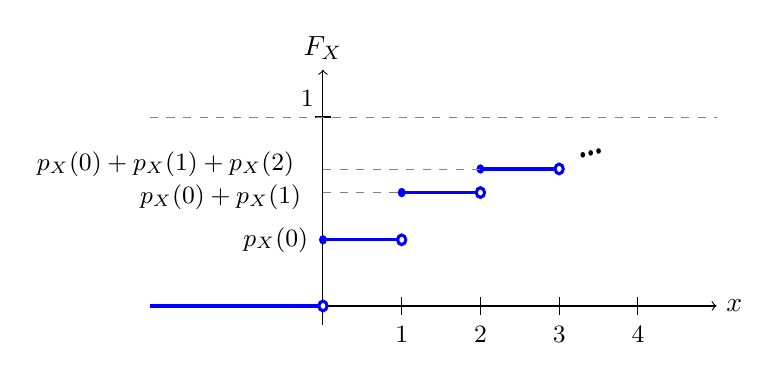
\begin{tikzpicture}[domain=0:4, yscale=1.2]
\draw[->] (-2.2,0) -- (5,0) node[right] {$x$};
\draw[->] (0,-0.2) -- (0,2.5) node[above] {$F_X$};
\draw (1,-0.1) -- (1,0.1);
\draw (2,-0.1) -- (2,0.1);
\draw (3,-0.1) -- (3,0.1);
\draw (4,-0.1) -- (4,0.1);

\draw[very thick,color=blue] (-2.2,0) -- (0,0);
\draw[very thick,color=blue] (0,0) circle (.05cm);
\fill[very thick,color=white] (0,0) circle (.03cm);

\fill[very thick,color=blue] (0,0.7) circle (.05cm);
\draw[very thick,color=blue] (0,0.7) -- (1,0.7);
\draw[very thick,color=blue] (1,0.7) circle (.05cm);
\fill[very thick,color=white] (1,0.7) circle (.03cm);

\fill[very thick,color=blue] (1,1.2) circle (.05cm);
\draw[very thick,color=blue] (1,1.2) -- (2,1.2);
\draw[very thick,color=blue] (2,1.2) circle (.05cm);
\fill[very thick,color=white] (2,1.2) circle (.03cm);
\draw[very thin,dashed,color=gray] (0,1.2) -- (1,1.2);

\fill[very thick,color=blue] (2,1.45) circle (.05cm);
\draw[very thick,color=blue] (2,1.45) -- (3,1.45);
\draw[very thick,color=blue] (3,1.45) circle (.05cm);
\fill[very thick,color=white] (3,1.45) circle (.03cm);
\draw[very thin,dashed,color=gray] (0,1.45) -- (2,1.45);


\draw (-0.1,2) -- (0.1,2);

\fill[very thick,color=black] (3.3,1.6) circle (.03cm);
\fill[very thick,color=black] (3.4,1.62) circle (.03cm);
\fill[very thick,color=black] (3.5,1.64) circle (.03cm);

\draw (-0.6,0.7) node {\small $p_X(0)$};
\draw (-1.3,1.15) node {\small $p_X(0)+ p_X(1)$};
\draw (-2,1.5) node {\small $p_X(0)+ p_X(1)+p_X(2)$};
\draw (1,-0.3) node {\small $1$};
\draw (2,-0.3) node {\small $2$};
\draw (3,-0.3) node {\small $3$};
\draw (4,-0.3) node {\small $4$};
\draw (-0.2,2.2) node {\small $1$};
	\draw[very thin,dashed,color=gray] (-2.2,2) -- (5,2);
\end{tikzpicture}


